\section{Experiment Setup}
\subsection{Motivation}
%todo: mover classical to traditional.
During Automated Program Repair (APR) activities, classical methods (based on heuristics or templates) often generate syntactically correct changes, but they fall short in the semantic and code style aspects (insert ref).

In this context, Large Language Models (LLMs) are capable of capturing code patterns and semantic context with high precision.
On the other hand, LLMs exhibit significant sensitivity to how their instructions (prompts) are phrased. Different instructions can alter the fidelity to the original style, the clarity of the patch, and the size of the modification, especially if little context is provided during the correction process (insert ref).

\subsection{Dataset}
% TODO: adicionar referencia de pytracebugs
The experiment uses the Pytracebugs dataset \cite{Pytracebugs}, which contains Python source codes from GitHub repositories at the granularity of function snippets and their corresponding Traceback errors; see the example below.
% TODO: referencia ao exemplo

\begin{figure}[h!]
    \centering
    \caption{An example of a single data point from the Pytracebugs dataset.}
    \label{fig:dataset-example}

    % (a) The Buggy Code
    \begin{lstlisting}[
        language=Python,
        frame=single,
        basicstyle=\ttfamily\small,
        title={a) Buggy Code Snippet (\texttt{before\_merge})},
        title_style=\bfseries,
        belowcaptionskip=-0.5em % Adjust spacing
        ]
def noise(self, value):
  self.noise_covar.initialize(value)
    \end{lstlisting}

    % (b) The Traceback Error
    \begin{lstlisting}[
        frame=single,
        basicstyle=\ttfamily\small,
        title={b) Traceback Error (\texttt{full\_traceback})},
        title_style=\bfseries,
        belowcaptionskip=-0.5em % Adjust spacing
        ]
import gpytorch
gl = gpytorch.likelihoods.GaussianLikelihood()
gl.initialize(noise=1)
Traceback (most recent call last):
File ""<stdin>"", line 1, in <module>
File "".../gpytorch/gpytorch/module.py"", line 89, in initialize
setattr(self, name, val)
File ""../lib/python3.6/site-packages/torch/nn/modules/module.py"", line 579, in __setattr__
object.__setattr__(self, name, value)
File "".../gpytorch/gpytorch/likelihoods/gaussian_likelihood.py"", line 63, in noise
self.noise_covar.initialize(value)
TypeError: initialize() takes 1 positional argument but 2 were given
    \end{lstlisting}

    % (c) The Fixed Code
    \begin{lstlisting}[
        language=Python,
        frame=single,
        basicstyle=\ttfamily\small,
        title={c) Fixed Code Snippet (\texttt{after\_merge})},
        title_style=\bfseries
        ]
def noise(self, value):
  self.noise_covar.initialize(noise=value)
    \end{lstlisting}
\end{figure}


%TODO: Adicionar exemplos de trabalhos publicados que utilizam como referencia o dataset proposto.
Some published works that use this dataset aim to study problems such as Vulnerability Detection \cite{zhao2024coding} and fault localization \cite{kulkarni2024graph}.

\subsection{LLM Models}
For the first experiment, four models were chosen. Two of these are open-source models specialized in code generation, considered state-of-the-art in this category: Qwen 2.5 coder 32b (instruct) \cite{hui2024qwen25codertechnicalreport} and Codestral 2501 \cite{Codestral_202501}. Additionally, two state-of-the-art, commonly used closed-source models of a relatively similar size were selected: Claude $3.5$ Sonnet and GPT $4o$ Model.

Esses modelos apesar de todos competitivos similarmente em benchmarks estruturados, diferem-se consideravelmente em questões de Preço durante a usabilidade.
Para referência o custo por token dos modelos escolhidos pode ser visto na tabela \ref{tab:model-tokens}
\begin{table}[h!]
\centering
\caption{Token usage price per model.}
\label{tab:model-tokens}
\begin{tabular}{|l|c|c|}
\hline
\textbf{Model} & \textbf{Input Tokens (1M)} & \textbf{Output Tokens (1M)} \\ \hline
Claude Sonnet 3.5 & \$3.0 & \$15.0 \\ \hline
Gpt 4o & \$2.5 & \$10 \\ \hline
Codestral 2501 & \$0.3 & \$0.9 \\ \hline
Qwen 2.5 Coder 32B Instruct & \$0.05 & \$0.20 \\ \hline
\end{tabular}
\end{table}
% todo addicionar gemini flas
%TODO melhorar a argumentação desses modelos
% Falar do tamanho dos modelos e da comparabilidade deles. Exibir ranking. Existem muitos, portanto qualquer escolha tem uma arbitrariedade. Não vamos todos no hugging faces.

% TODO trazer artigos que divulgam esses modelos.


\subsection{Prompts updated}

To test the model's sensitivity to the prompt's instructions, all prompts were formatted 
using a consistent template, shown in Listing \ref{lst:prompt-template}. This structure ensures 
that each model receives the context—buggy code and traceback error—in a clear, delimited 
format, and is explicitly asked to return only the corrected code.

% The 'figure' environment helps manage the placement and captioning of the listing.
\begin{figure}[h!]
% This is the crucial line that starts the code block.
% The formatting options are placed in the square brackets.
\begin{lstlisting}[
    caption={The general template used for all prompts.},
    label={lst:prompt-template},
    basicstyle=\ttfamily\small,
    frame=single,
    breaklines=true
]
{{ instruction_prompt }}

### BUGGY CODE:
{{ buggy_code }}

### ERROR:
{{ traceback_error }}

### RETURN ONLY THE CORRECTED CODE BELOW:

IMPORTANT: Return ONLY the corrected/requested code. Do not include any explanations, comments about the changes, or other text. Just return the pure code.

\end{lstlisting} % This line correctly ends the code block.
\end{figure}
% It clearly isolates the variable you are testing.
\begin{table}[h!]
\centering
\caption{Instruction variations for the \texttt{instruction\_prompt} variable.}
\label{tab:prompt-instructions}
\begin{tabular}{|l|p{0.55\textwidth}|p{0.15\textwidth}|}
\hline
\textbf{Prompt ID} & \textbf{Instruction Text} & \textbf{System Prompt} \\ \hline
P1 (Baseline) & You are a helpful assistant that corrects the code based on the traceback error. & False. \\\hline
P2 (Style-aware) & You are a helpful assistant that corrects the code based on the traceback error. You must respect the original code structure and the original code style. & False. \\ \hline
P3 (System Prompt) & You are a helpful assistant that corrects the code based on the traceback error. & True. \\ \hline
\end{tabular}
\end{table}
The core of the experiment lies in the variation of the \texttt{instruction\_prompt} placeholder and the addition of system prompt. 
We designed three distinct instructions, which we will refer to as P1 (Baseline) and P2 (Style-aware) and P3 (System Prompt), 
to evaluate the impact of a more detailed directive. The specific text for each instruction 
is detailed in Table \ref{tab:prompt-instructions}.

\subsection{Experiment tracking}
For each of the 4 models, 300 responses were executed for each of the prompts, totaling 4 x 300 x 3 = 3600 responses. For each response, the following metrics were evaluated: AST, AST-Normalized, CodeBLEU, N-gram match, Weighted N-gram match, Dataflow Match.
Each metric was compared against both the original (buggy) code and the ground truth correction.


\subsection{Implementation Details}
\label{sec:implementation-details}

All API calls to the proprietary models (GPT-4o and Claude 3.5 Sonnet) and the open-source models (Qwen 2.5 and Codestral) were managed through the \textbf{OpenRouter} API aggregation service. This approach was chosen to ensure a consistent and reproducible experimental setup across all models from a single interface.

The specific model identifiers used on the platform are listed below. To ensure that the results were as deterministic as possible and to facilitate a fair comparison, the generation parameters were kept constant for all API calls: a \textbf{temperature of 0} and a \textbf{top\_p of 1.0} were used. All experiments were conducted in \textbf{July 2025}.

\begin{itemize}
    \item \texttt{openai/gpt-4o}
    \item \texttt{anthropic/claude-3.5-sonnet}
    \item \texttt{qwen/qwen-2.5-coder-32b-instruct} 
    \item \texttt{mistralai/codestral-2501}
\end{itemize}


% Manipuladores subatuados diferem dos totalmente atuados pois são equipados com um número de atuadores que é sempre menor que o número de \gls{graus_liberdade}. Portanto, nem todos os \gls{graus_liberdade} podem ser controlados ativamente ao mesmo tempo \cite{Sbornian2004}. Por exemplo, com um manipulador planar de 3 juntas equipado com dois atuadores, ou seja, duas juntas ativas e
% uma passiva, pode-se controlar ao mesmo tempo duas das juntas a qualquer instante, mas não todas. Para controlar todas as juntas de um manipulador subatuado, deve-se usar um controle sequencial. Este princípio foi provado pela primeira vez por {arai} usando  argumentos dinâmicos linearizados \cite{Joea2003}, e é a base para a modelagem no espaço das juntas e no espaço Cartesiano. A Tabela \ref{minhatab} apresenta os resultados \cite{Assenmacher1993,Silberschatz1991,Caromel1998}.

% \begin{table}
% \caption{Exemplo de uma Tabela}
% \label{minhatab}

% \center
% \begin{tabular}{cccc}
%   % after \\: \hline or \cline{col1-col2} \cline{col3-col4} ...
%   \hline
% 	Parâmetro & Unidade & Valor da simulação & Valor experimental   \\
% 	\hline
%   Comprimento, \gls{comprimento} & $m$ &  $8,23$  & $8,54$ \\
%   Altura, \gls{altura} & $m$     &  $29,1$ & $28,3$\\
% 	Velocidade, \gls{velocidade} & $m/s$  &  $60,2$ & $67,3$\\
% 	\hline
% \end{tabular}
% \end{table}

% Devido ao fato de que no máximo $n_{a}$ coordenadas generalizadas (ângulos das juntas ou variáveis cartesianas) podem ser controladas num dado instante, o vetor de coordenadas generalizadas é dividido em duas partes, representando as coordenadas generalizadas ativas e as coordenadas generalizadas passivas \cite{Callaghan1995}.

% \begin{figure}[ht]
% \centering
% 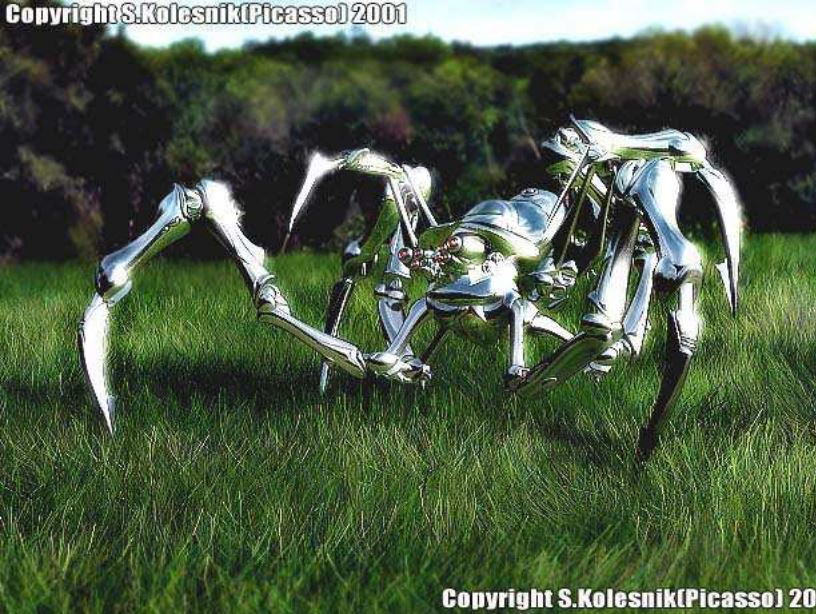
\includegraphics[width=0.75\textwidth]{Cap2/spiderrobot}
% \caption{Cupim cibernético.}\label{FDIII}
% \end{figure}

% Considerando um robô manipulador rígido, malha aberta, e de $n$-juntas em série. Seja $q$ a representação de seu vetor de posição angular das juntas  e $\tau$ a representação de seu vetor de torque. A equação dinâmica pelo método de
% Lagrange é dada por:
% \begin{equation} \label{eq:lagr1}
% \frac{d}{dt} \left( \frac{\partial L}{\partial \dot{q}} \right) -\frac{\partial L}{\partial q}=\tau^{T}.
% \end{equation}
% O Lagrangiano $L$ é definido como a diferença entre as energias cinética e potencial do sistema:
% \begin{equation} \label{L}
% L=T-P
% \end{equation}

% A energia cinética total dos ligamentos é representada:
% \begin{equation} \label{energT}
% T=\frac{1}{2}\dot{q}^{T}M(q)\dot{q}
% \end{equation}
